\documentclass[a4paper,12pt,twoside]{article}

%===========PACOTES
\usepackage[body={160mm,235mm}]{geometry}
%\usepackage[portuguese]{babel}
\usepackage{a1}
\usepackage[english]{babel}
\usepackage[latin1]{inputenc} %permite o uso de acentos
%\usepackage[dvips]{color}
\usepackage{amsfonts,amssymb}
%\usepackage{epsfig}
\usepackage{amsmath}
\usepackage{graphicx}	
\usepackage{float}
\usepackage[pdftex]{hyperref}
\usepackage{url}
\usepackage{color}

% makeidx
\usepackage{makeidx}
% make index
\makeindex
%\usepackage[pdftex]{graphicx}


\def\mapright#1#2#3{\smash{\mathop{\hbox to
#3{\rightarrowfill}}\limits^{#1}_{#2}}}

\def\mapleft#1#2#3{\smash{\mathop{\hbox to
#3{\leftarrowfill}}\limits^{#1}_{#2}}}

\def\mapright#1#2{\smash{\mathop{\hbox to 0.90cm{\rightarrowfill}}\limits^{#1}_{#2}}}
\def\mapleft#1#2{\smash{\mathop{\hbox to 0.90cm{\leftarrowfill}}\limits^{#1}_{#2}}}

\def\mapleftright#1#2{\smash{\mathop{\hbox to 0.80cm{\leftarrowfill \rightarrowfill}}\limits^{#1}_{#2}}}
\def\ext{\times \! \vrule depth0pt height5pt width0.35pt}

\def\H{\mathcal H}
\def\D{\mathcal D}
\def\B{\mathcal B}
\def\C{\mathbb C}
\def\R{\mathbb R}
\def\S{\mathbb S}
\def\U{\mathcal U}
\def\Z{\mathbb Z}

\title{The $\kappa_r$-version of the WRT$_r$-invariants, monochromatic 3-connected blinks 
and evidence for a conjecture on their induced 3-manifolds
\footnote{2010 Mathematics Subject Classification: 
05C85 and 05C83 (primary), 57M27 and 57M15 (secondary)}} 
\author{S�stenes L. Lins, Cristiana G. Huiban, Lauro D. Lins}

\date{\today}


\begin{document}


\maketitle

\begin{abstract}
A {\em blink} is a plane graph with a bicoloration of its edges into black and gray edges.
Subtle equivalence class of blinks are in 1-1 correspondence with closed, 
oriented and connected 3-manifolds up to orientation preserving homeomorphisms,
see \url{http://arxiv.org/abs/1305.4540}, \cite{lins2013B}.
Switching black and gray in a blink $B$ reverses the orientation obtaining -$B$.
The dual of the blink $B$ in the sphere $\mathbb{S}^2$ is denoted by $B^ \star$. Blinks 
$B$ and $-B^\star$ induce the same 3-manifold.
This paper concludes (up to a single uncertainty) the topological 
classification of $T_{16}$, the set of 381 monochromatic 3-connected blinks 
up to 16 edges. The classification justifies the Conjecture 
that if $B' \notin \{B,-B^\star\}$, then $B$ and $B'$ induce distinct 3-manifolds.
The isomorphism problem for blinks is solvable by an $O(n^2\log n)$-algorithm.
\end{abstract}

\section{Introduction}
It is well known that a 3-connected graph has a unique pair of enantiomorphic
embeddings in the 2-sphere \cite{welsh2010matroid}. The present paper
suggests a manifestation of this fact in closed oriented connected 3-manifolds
induced by 3-connected monochromatic blinks, restricting the 1-1 correspondence 
of  \url{http://arxiv.org/abs/1305.4540}, \cite{lins2013B} to that blinks.
\subsection{The set of 381 blinks $T_{16}$}

The set $T_{16}$ with 381 blinks is explicitally generated and displayed in
\url{http://arxiv.org/arXiv:math/0702057},\cite{lins2007blink}.
In the same work, the classification up to oriented homeomorphisms 
for the 3-manifolds induced by blinks in $T_{16}$ was nearly performed by, $\kappa_r$, $r=3,\ldots 8$, the 
Kauffman-Lins version (\cite{kauffman1994tlr}) of the WRT-invariants, leaving exactly 11 doubts. 
In section \ref{sec:kappar}, for completude, we give the full definition and an associated 
combinatorial algorithm
to obtain these invariants using solely the blink as input.
Ten of eleven doubts are solved in the present work.
Here are the numbers of monochromatic 3-connected blinks up to 16 edges, indexed
by a fixed number of edges:
$6\mapsto 1, 8\mapsto 1, 9\mapsto 1, 10\mapsto 2, 
11\mapsto 2,\ 12\mapsto 9, 13\mapsto 11, 14\mapsto 36, 15 \mapsto 76, 16\mapsto 242,$ so that
$T_{16}$ has a total of 381 blinks. Dual blinks are not filtered in \cite{lins2007blink}. 
This was on purpose to 
control the generation algorithms. When we perform the $\kappa_r$-classification, these dual
blinks $(\pm B, \mp B^\star)$ must appear, as they do, together. As a matter of fact we only 
draw one of $\pm B$, the other is obtained by exchanging black and gray edges. The effect 
of taking the negative blink in $\kappa_r(B)$ is to conjugate the complex number:
for all blinks $B$, $\kappa_r(B) = \overline{\kappa_r(-B)}$ and 
$\kappa_r(B) = \kappa_r(-B^\star)$.

The clarification of these doubts answers all but one of the challenges posted 
in \url{http://arxiv.org/abs/1305.2617}, \cite{lins2013}.
From \url{http://arxiv.org/arXiv:math/0702057},
\cite{lins2007blink} we know that among all 3-connected monochromatic blinks
up to 16 edges, forming the set $T_{16}$, 
there are only eleven that has a $HG8QI$-class with more than
one pair $(B,-B^\star)$. These are the following:
(1) $14^t_{24}$,\ 
(2) $15^t_{16}$,\  
(3) $15^t_{19}$,\  
(4) $15^t_{22}$,\  
(5) $16^t_{42}$,\  
(6) $16^t_{56}$,\  
(7) $16^t_{140}$,\  
(8) $16^t_{141}$,\  
(9) $16^t_{142}$,\  
(10) $16^t_{149}$,\  
(11) $16^t_{233}$.
All the other pairs of blinks $(B,-B^\star)$ in $T_{16}$ are 
complete graphical invariants for their induced 3-manifolds.
We show that all but one (which remains unknown) of these classes 
break into two classes of homeomorphisms.
The distinction in 9/10 cases is obtained by a combined action of the systems SnapPy, GAP and Sage.
We find all the homeomorphisms of the fundamental group of the induced 3-manifold onto 
the symmetric group $S_k$, for small adequate $k$. Using them then 
we compute the homology of the cover 3-manifolds
based in these homeomorphisms of the induced 3-manifolds. 
Even though we could not find covers for $HG8QI$-class $16_{149}$
the computation of volumes is quick in SnapPy and 
shows that the two members of this class are not homeomorphic. 
Thus, using covers and volumes we were able to distinguish all the $HG8QI$-classes,
except $16^t_{140}$, which remains a big challenge. However, to conform with 
the other  $HG8QI$-classes, we conjecture that it also breaks into two homeomorphism classes.

\subsection{Acknowledgments}
We are indebted to Marc Culler who kindly provided clues on how to install and 
how to use SnapPy and first found some of the distinguishing covers that follow.
The first author thanks the financial support of CIn/UFPE and CNPq.

\section{$\kappa_r$: the Kauffman-Lins version of the WRT-invariants}
\label{sec:kappar}
To each blink $B$ and each integer $r \ge 3$ we will associate a complex number
$\kappa_r(B)$. If $B'$ is another blink obtained from 
$B$ by moves in the coin calculus  \url{http://arxiv.org/abs/1305.4540}, \cite{lins2013B},
then $\kappa_r(B)=\kappa_r(B')$. Therefore, $\kappa_r$ is an 
{\em invariant of closed, orientable, connected 3-manifolds}.
The invariant $\kappa_r$ was obtained and justified in the 
Kauffman-Lins monography \cite{kauffman1994tlr}. Its invariance relies in the 
properties of Kauffman's bracket and on the algebraic properties of the Temperley-Lieb algebra.
Subsequently it was realized that this invariant is one of the manifestations of 
the Witten-Reshetikhin-Turaev invariants. 
Originally these invariants were found by Witten in the late 1980's using a physical formalism that was
not perfectly mathematically satisfactory. Witten's result broke the prejudice that
good invariants of 3-manifolds did not exist. Shortly after, some eastern european researchers as
Turaev, Viro, Reshetikhin, Kirillov and others, produced full mathematical proofs of the invariance
of Witten's results using quantum groups,
\cite{witten1989quantum,reshetikhin1991invariants,turaev1992state,kirillov1993orbit}.
However, quantum groups is a rather complicated subject and Kauffman-Lins 
using some ideas of Lickorish (invariance of second of Kirby's moves (\cite{lickorish1991three}) 
via the 
Temperley-Lieb algebra and cubic graphs embedded into 3-space --- see also 
page 144 of Kauffman-Lins monography,
and Turaev (shadow world (\cite{turaev1994quantum}), which makes possible to 
combinatorialize the whole situation), 
provided the $\kappa_r$-invariant, which demands much less
machinery to be understood. It is our intention here to provide a 
complete recipe for obtaining the $\kappa_r$-invariant in a way to be simply understood
by a combinatorially inclined reader. Our idea is to make it available for the Combinatorics 
community these strong and mysterious
quantum invariants: an infinite sequence of complex numbers which are deterministically
possible to assigned to blinks up to the coin calculus and to (they are the same, there is
a 1-1 correspondence) 3-manifolds up to orientable 
homeomorphisms. The invariance issue will remain untouched in this work;
it is treated in detail in \cite{kauffman1994tlr}.

\begin{figure}[H]
\begin{center}
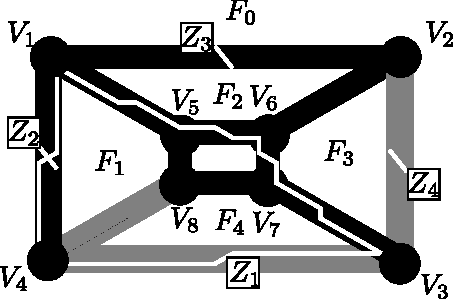
\includegraphics[width=6.0cm]{A.figs/zigzagcube.pdf} 
\caption{\sf The zigzags of a blink $B$ and the domain of an $r$-state $\sigma$: 
an $r$-state $\sigma$ is a function from $\mathbb{D}(B)$ to $\mathcal{I}m(\sigma)=\mathcal{I}=
\{3,\ldots,r-2\}$;
a zigzag in a plane graph is a closed path that alternates taking the leftmost turn
and the rightmost turn at each vertex; zigzags in general surfaces (orientable and non-orientable)
are studied in \cite{lins1982graph}.
the bipartition of the edge colors of the blink plays no role in the definition of the zigzags;
a zigzag traverses at most twice each edge,
so that the total number of edges traversed by the set of zigzags is exactly $2n$, where $n$ is the 
number of edges of the blink;
The domain of $\sigma$ is the union of its vertices, the faces and the 
zigzags of the blink $B$. In the example the domain is
$\mathcal{D}(\sigma)=\{V_1,V_2,V_3,V_4,V_5,V_6,V_7,V_8,F_0,F_1,F_2,F_3,F_4,F_5,Z_1,Z_2,Z_3,Z_4\}$.
}
\label{fig:zigzagcube}
\end{center}
\end{figure} 


\subsection{The ingredients for computing $\kappa_r$}
\label{subsection:kappaerre}
This section is a reformulation of Chapter 7 of \cite{lins1995gca}.
The invariance depends on the Jones polynomial and on the Temperley-Lieb algebra. 
The complete theory is developed from scratch in \cite{kauffman1994tlr}.

Let $A=e^{\frac{\pi i}{2r}}$ be the ``first'' primitive $4r$-th root of unity, $r \ge 3$,  and
${\cal I} = \{0,1,...,r-2\}$. For $n$ in ${\cal I}$, let
$$\Delta_n = (-1)^n\frac{\textstyle A^{2n+2}-A^{-2n-2}}
{\textstyle A^2-A^{-2}}, \hspace{10mm}
[n] = \frac{\textstyle A^{2n}-A^{-2n}}{\textstyle A^2-A^{-2}}=
(-1)^{n-1}\Delta_{n-1}.$$
Letting $q=A^2$, for reasons inherited from
the physics we call $[n]$ the
{\em $q$-deformed
quantum integer}\index{$q$-deformed!quantum integer}
and
$[n]! = \prod_{0 \le m \le n} [m]$
the
{\em $q$-deformed
quantum factorial}\index{$q$-deformed!quantum factorial}.
Note that even though $A$
is complex, $\Delta_n$ and $[n]$ assume only real values.
Three numbers $a,b,c \in {\cal I}$ form an
{\em $r$-admissible triple}\index{admissible triple}
if $a+b+c \le 2r-4$ and $a+b-c, b+c-a, c+a-b$ are non-negative and even.
Let $\theta: \mathcal{I}^3 \mapsto \mathbb{R}$, defined on the $r$-admissible
triples by means of
$$
\theta(a,b,c)=\frac{\textstyle (-1)^{m+n+p}[m+n+p+1]! [n]! [m]! [p]!}
{\textstyle [m+n]! [n+p]! [p+m]!}\ , \mbox{where}
$$ 
$m= (a+b-c)/2, n=(b+c-a)/2, p=(c+a-b)/2.$
We define $\theta(a,b,c)=0$ if $(a,b,c)$ fails to be $r$-admissible.

Let $\lambda: \mathcal{I}^3 \mapsto \mathbb{C}$, be defined on the $r$-admissible
triples by
$$
\lambda(a,b,c)=\lambda^{ab}_c=
(-1)^{(a+b-c)/2}A^{[a(a+2)+b(b+2)-c(c+2)]/2}
$$
We let $\lambda^{ab}_c = 0$ if $(a,b,c)$ fails to be $r$-admissible.
Finally, define $Tet: \mathcal{I}^6 \mapsto \mathbb{R}$, as follows.
If $(\alpha,\beta,\phi)$, $(\alpha,\delta,\epsilon)$, 
$(\gamma,\delta,\phi)$, $(\beta,\gamma,\epsilon)$ are $r$-admissible,
define


$$Tet(\alpha,\beta,\gamma,\delta,\epsilon,\phi)=
Tet\left[
\begin{matrix}
\alpha&\beta&\epsilon \cr 
\gamma&\delta&\phi\cr
\end{matrix}
\right]
=\frac{\mathcal
{I}nt!}{\mathcal{\epsilon}xt!}\sum_{m\leq s\leq
M}\frac{(-1)^s[s+1]!}{\prod_i[s-a_i]!\prod_j[b_j-s]!}$$ 
where,
$$\begin{array}{rcl}
{\cal I}nt!&=&\prod_{i,j}[b_j-a_i]!\\ [0.2cm]
{\cal \epsilon}xt!&=&[\alpha]![\beta]![\gamma]![\delta]![\epsilon]![\phi]!\\ [0.2cm]
a_1&=&\frac{1}{2}(\alpha+\delta+\epsilon)\qquad b_1=\frac{1}{2}(\beta+\delta+\epsilon+\phi)\\ [0.2cm]
a_2&=&\frac{1}{2}(\beta+\gamma+\epsilon)\qquad b_2=\frac{1}{2}(\alpha+\gamma+\epsilon+\phi)\\ [0.2cm]
a_3&=&\frac{1}{2}(\alpha+\beta+\phi)\qquad b_3=\frac{1}{2}(\alpha+\beta+\gamma+\delta)\\ [0.2cm]
a_4&=&\frac{1}{2}(\gamma+\delta+\phi)\qquad m\!=\!\max\{a_i\}\quad M\!=\!\min\{b_j\}\\
\end{array}$$
If one of the four triples above fails to be $r$-admissible, define
the value of $Tet$ as null.
These are all the algebraic
ingredients we need to define a function $\kappa_r$
on a $B$, where $r\ge 3$ is an integer.

\begin{figure}[H]
\begin{center}
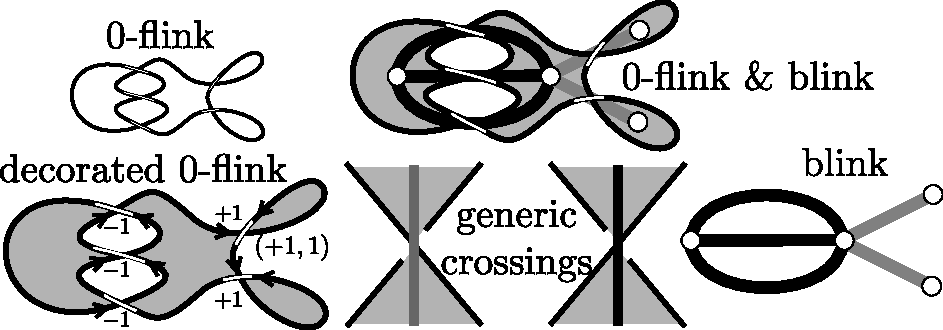
\includegraphics[width=9.0cm]{A.figs/flinkblink.pdf} 
\caption{\sf From 0-flink to blink and back: 
the projection of any 0-flink can be 2-face colorable into white and gray with the infinite
face being white so that each sub-curve between two crossing have their incident 
faces receiving distinct
colors. The above figure shows how to transform a 0-flink projection into a blink (with thicker edges
than the curves representing the link projection). 
The vertices of the blink are distinguished fixed
points represented by white disks in the interior of the gray faces. 
Each crossing of the link projection becomes an edge in the corresponding blink, 
An edge of the blink is gray if the upper strand 
that crosses it is from northwest to southeast, it is black if the the upper strand 
that crosses it is from northeast
to southwest. The inverse procedure
is clearly defined. In fact, the 0-flink is the so called {\em medial map} of the blink.
Thus we have a 1-1 correspondence between 0-flinks
and blinks.}
\label{fig:flinkblink}
\end{center}
\end{figure} 

We define a state sum $\kappa_r'(B)$ which out to be an invariant under Kirby's
second move, the {\em band move} or the {\em handle slide move}, \cite{kirby1978calculus},
see also page 144 of \cite{kauffman1994tlr} or  \url{http://arxiv.org/abs/1305.4540}, \cite{lins2013B}.
Each $r$-state contributes with one monomial for 
$\kappa'_r(B)$. A face of a connected blink is a connected component of 
complement $\mathbb{R}^2 \backslash B$.
There is a distinguished face (the infinite one) 
which is mapped to 0 by any admissible $r$-state $\sigma$.
With this restriction, $\kappa_r'$ is clearly multiplicative,
$\kappa'_r(B \cup B') = \kappa_r'(B) \times \kappa_r'(B')$
for disjoint blinks $B$ and $B'$. 

In obtaining the ingredients for the factors 
the bipartition of the edge set of the blink is disregarded, except for the 
$\lambda(a,b,c)$'s. They are also the only terms which are indeed complex:
$Tet(\alpha,\beta,\gamma,\delta,\epsilon,\phi)$, $\theta(a,b,c)$ and $\Delta_n$ are reals.  A
{\em state is $r$-admissible}\index{$r$-admissible!state}
if \label{fig:edgeanglefactors} the triples of numbers associated
to the incident trios (vertex,face,zigzag) is $r$-admissible. If a state is not admissible,
its value is declared to be 0.
From each $r$-state we
produce a complex number and the value $\kappa'_r(B)$ 
is the sum of all its {\em $r$-admissible} states.
Having invariance under Kirby's band move,
all that we need to have a 3-manifold invariant is to define
$$\kappa_r(B) = \kappa_r'(B) \left(\sin(\frac{\pi}{r}) \sqrt{\frac{2}{r}}\right)^{|F|+1}
\left(
(-1)^{r-2} e^{\frac{3 i \pi(r-2)}{4r}}\right)^{-n(F)}.$$
In this formula, $F$ is the 0-flink associated to $B$, $|F|$ is the number of components
of $F$, $n(F)$ is the number of positive eigenvalues minus the number of negative eigenvalues
of the {\em linking matrix} of $F$, which is easily obtained from the 0-flink $F$, see
page 254 of \cite{lins1995gca}. 
The factor we introduce to go from $\kappa_r'(B)$ to $\kappa_r(B)$
compensates for the multiplicative change that happens in the state sum $\kappa_r''(B)$ when
we introduce an isolated gray or black edge in the blink: this is the blink manifestation
of Kirby's move of type 1. With these definitions we it is possible to prove 
(see pages 146\cite{kauffman1994tlr}) that for all $r \ge 3$,
$$\kappa_r(\circ)=1 \rm{\ and\ }
\kappa_r(\circ \hspace{-0.5mm} \text{---} \hspace{-0.5mm} \circ)=\sin(\frac{\pi}{r}) \sqrt{\frac{2}{r}},$$
where $\circ$ denotes the isolated vertex blink, inducing $\mathbb{S}^2\times \mathbb{S}^1$ and
$\circ$\hspace{-0.5mm}---\hspace{-0.5mm}$ \circ$ denotes the isolated single edge 
blink inducing $\mathbb{S}^3$.
See Fig. \ref{fig:edgeanglefactors} to complement this material. 

\begin{figure}[H]
\begin{center}
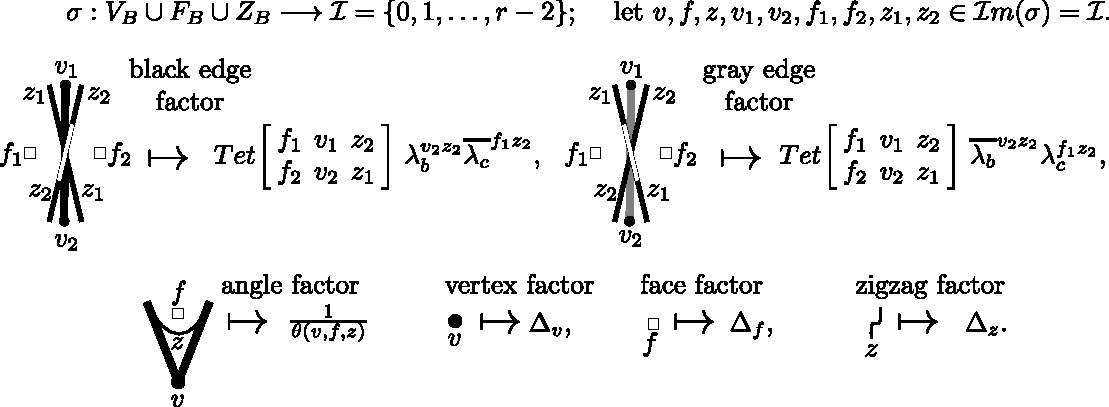
\includegraphics[width=16.0cm]{A.figs/edgeanglefactors.pdf} 
\caption{\sf 
The {\em ingredients} and the {\em sites} for computing the $\kappa_r$-invariant from a blink $B$:
black edge, gray edge, angle, vertex, face and zigzag are sites to have associated 
factors depending on a fixed $r$-state
$\sigma$ in the computation of the $\kappa_r$-invariant; it is obtained
from blink $B$ as follows: {\em a state} $\sigma$ is a function from the union
of the vertices, the faces and the zigags of $B$ to an alphabet $\mathcal{I}=\{0,1,\ldots r-2\}$.
The {\em value of the $r$-state} is the product  of complex numbers in 1-1 correspondence with 
the factors for the black edges, the gray edges, the angles, 
the vertices, the faces and the zigzags; the value of $\kappa'_r(B)$ is the sum 
of the $r$-admissible (as defined in Subsection \ref{subsection:kappaerre}) 
states of $B$; in the above figure,
$v,f,z,v_1,v_2,f_1,f_2,z_1,z_2$ are the images under 
the specific $r$-state $\sigma$ of, respectively, 
$V,F,Z,V_1,V_2,F_1,F_2,Z_1,Z_2$; the evaluations of the ingredients for the 
factors, $Tet(\alpha,\beta,\gamma,\delta,\epsilon,\phi)$, 
$\lambda_{ab}^c$, $\overline{\lambda}_{ab}^c$,  $\theta(a,b,c)$, $\Delta_n$ are detailed in Subsection
\ref{subsection:kappaerre}; there are symmetries in the situation which
imply that the edge factors are invariant under a half turn rotation. There is an adequate factor
which multiplied by $\kappa'_r(B)$  produce a 3-manifold invariant $\kappa_r(B)$.
See Subsection \ref{subsection:kappaerre}.
}
\label{fig:edgeanglefactors}
\end{center}
\end{figure} 


\section{Solving 10/11 $HG8QI$-classes as non-homeomorphic pairs}

An $HGnQI$-class of blinks is the set of blinks inducing a 3-manifold
with the same homology and the same $\kappa_r$ invariants, for $r=3,\ldots,n$.
We have used a combination of the softwares SnapPy/GAP/Sage to prove that
that 10 out of the 11 pairs of blinks in these $HG8QI$-classes induce
distinct 3-manifolds. The only exception was $16_{140}$ which remains unconquered.
We conjecture that it also breaks into two classes of homeomorphisms.
In the figures of this section we present both the blink and its associated 0-flink
(defined in see \url{http://arxiv.org/abs/1305.4540}, \cite{lins2013B}). However,
the 0-flinks and its pair of surgery coefficients attached to each component of 
the 0-flink (good for input in the SnapPy) are
redundant, as they are implied by the small blink displayed at the southwest of each
0-flink. All the blinks are monochromatic, formed by black edges only. This corresponds 
to having only alternating 0-flinks. The running time of SnapPy/GAP/Sage for 
the 11 pairs varies a lot:
$14^t_{24} \mapsto  0m29.01s$,
$15^t_{16} \mapsto  2m17.75s$,
$15^t_{19} \mapsto  639m52.46s$,
$15^t_{22} \mapsto  125m51.74s$,
$16^t_{42} \mapsto  0m4.98s$,
$16^t_{56} \mapsto  0m2.63s$,
$16^t_{140} \mapsto  \infty$,
$16^t_{141} \mapsto  0m1.18.90s$,
$16^t_{142} \mapsto  233m453.92s$,
$16^t_{149} \mapsto  34m7.37s$,
$16^t_{233} \mapsto  1m5.63s$. In only one case, $16^t_{140}$, we report an $\infty$ because the case took
more than three days, inconclusively. The status of $16^t_{140}$ remains unknown.

\subsection{Distinguishing the 2 members of the $HG8QI$-class  $14^t_{24}$}
\begin{figure}[H]
\begin{center}
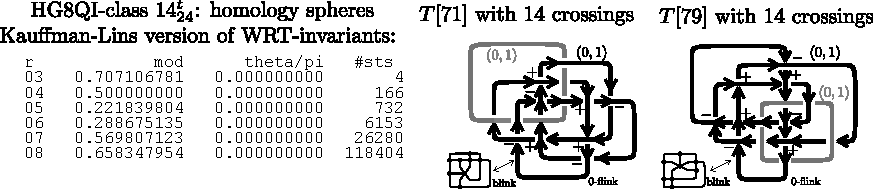
\includegraphics[width=16cm]{A.figs/T14_24.pdf} 
\caption{\sf Distinction on the $HG8QI$-class $14^t_{24}$:
We show the surgery coefficient pairs attached to each of the 0-flink components. These are determined by the 
blink. Covers of degree 5 perform the distinction. Homology of the three 5-covers of $T[71]$: $[Z/3 + Z/3 + Z/3 + Z/3, Z/63 + Z/63, Z/132 + Z/132]$.
Homology of the three 5-covers of $T[79]$: $[Z/3 + Z/3 + Z/3 + Z/3, Z/213 + Z/213, Z/432 + Z/432]$.
Therefore $T[71]$ and $T[79]$ induce non-homeomorphic 3-manifolds. By the 1-1 correspondence of 
\cite{lins2013B} we identify the blink and its induced 3-manifold.
Note that the volumes (as the Kauffman-Lins version of the WRT-invariants) do not distinguish:
volume of $T[71]$ --- 24.8073697340, volume of $T[79]$ --- 24.807369734. Sage is the front end of the
system; it calls SnapPy and GAP. Sage Execution Time (CPU time 0m0.42s, Wall time 0m29.01s).
}
\label{fig:T14_24}
\end{center}
\end{figure} 

\subsection{Distinguishing the 2 members of the $HG8QI$-class  $15^t_{16}$}
\begin{figure}[H]
\begin{center}
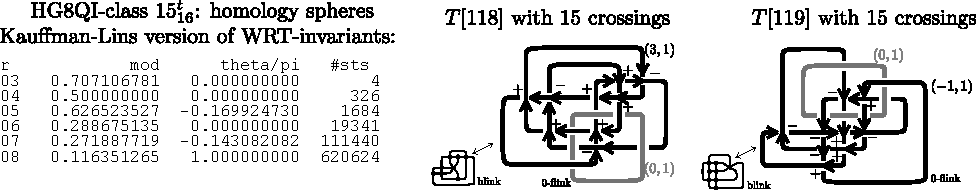
\includegraphics[width=16.0cm]{A.figs/T15_16.pdf} 
\caption{\sf Distinction on the $HG8QI$-class $15^t_{16}$:
Homology of the four 5-covers of $T[118]$: $[Z/229773, Z/1110327, Z/3018207, Z/3699687]$.
Homology of the four 5-covers of $T[119]$: $[Z/3 + Z/1299909, Z/126627, Z/1052067, Z/4117827]$.
Therefore $T[118]$ and $T[119]$ induce non-homeomorphic 3-manifolds. 
Note that the volumes (as the Kauffman-Lins version of the WRT-invariants) do not distinguish:
volume of $T[118]$ ---28.375305555, volume of $T[119]$ --- 28.3753055549. 
Sage Execution Time (CPU time 0m1.55s, Wall time 2m17.75s). 
}
\label{fig:T15_16}
\end{center}
\end{figure} 

\subsection{Distinguishing the 2 members of the $HG8QI$-class  $15^t_{19}$}
The $HG8QI$-class $15_{19}$ provided us 
with an example of the toughness of the computation
involved to obtain the coverings. It took SnapPy/GAP/Sage more than 10 hours
to obtain the (reported) 20 coverings.
\begin{figure}[H]
\begin{center}
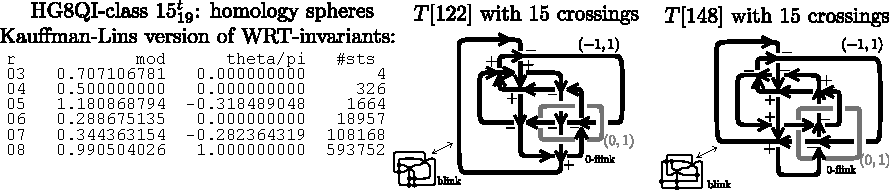
\includegraphics[width=16.0cm]{A.figs/T15_19.pdf} 
\caption{\sf Distinction on the $HG8QI$-class $15^t_{19}$:
Homology of the twenty 6-covers of
$T[122]$: 
$[
 Z/2 + Z/2 + Z/15486,
 Z/2 + Z/2 + Z/15486,
 Z/2 + Z/894,
 Z/2 + Z/894,
 Z/3 + Z/3 + Z/732,
 Z/3 + Z/3 + Z/732,
 Z/3 + Z/3 + Z/6552,
 Z/3 + Z/3 + Z/6552,
 Z/4 + Z/12,
 Z/4 + Z/12,
 Z/6 + Z/402,
 Z/6 + Z/402,
 Z/24 + Z,
 Z/24 + Z,
 Z/531,
 Z/531,
 Z/549,
 Z/549,
 Z/4716,
 Z/4716]$.
Homology of the twenty 6-covers of $T[148]$: 
$[Z/2 + Z/2 + Z/114,
 Z/2 + Z/2 + Z/384,
 Z/2 + Z/966,
 Z/3 + Z/3 + Z/51,
 Z/3 + Z/3 + Z/1302,
 Z/3 + Z/24 + Z,
 Z/6 + Z/6 + Z/444,
 Z/6 + Z/138,
 Z/6 + Z/150,
 Z/6 + Z/162,
 Z/6 + Z/450,
 Z/6 + Z/4842,
 Z/8 + Z/24,
 Z/18 + Z/450,
 Z/1341,
 Z/4356,
 Z/4866,
 Z/11025,
 Z/66402,
 Z/71496]$.
Therefore $T[122]$ and $T[148]$ induce non-homeomorphic 3-manifolds. 
Note that the volumes (as the Kauffman-Lins version of the WRT-invariants) do not distinguish:
volume of $T[118]$ ---27.670218370, volume of $T[119]$ --- 27.670218370. 
Sage Execution Time (CPU time 2m8.60s, Wall time 639m52.46s).
% Relative to $15_{19}^t$ we report a mismatch with M. Culler computations.
% He got 213 6-covers for $T[122]$ and 211 6-covers for $T[148]$.
% See the Conclusion Section in \url{http://arxiv.org/abs/1305.5590}, \cite{lins2013C}. Probably
% the mismatch is on the input surgery coefficients.
}
\label{fig:T15_19}
\end{center}
\end{figure} 

\subsection{Distinguishing the 2 members of the $HG8QI$-class  $15^t_{22}$}
\begin{figure}[H]
\begin{center}
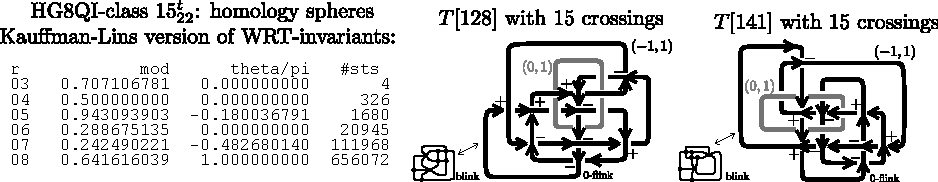
\includegraphics[width=16.0cm]{A.figs/T15_22.pdf} 
\caption{\sf Distinction on the $HG8QI$-class $15^t_{22}$:
Homology of the fifteen 6-covers of $T[128]$: $[Z/2 + Z/162,
 Z/2 + Z/234,
 Z/2 + Z/414,
 Z/2 + Z/1086,
 Z/3 + Z/3 + Z,
 Z/3 + Z/6 + Z + Z,
 Z/3 + Z/6 + Z + Z,
 Z/3 + Z/6 + Z/18 + Z/720,
 Z/3 + Z/6 + Z/18 + Z/720,
 Z/6 + Z/6 + Z/1296,
 Z/6 + Z/6 + Z/10800,
 Z/9,
 Z/207,
 Z/5571,
 Z/5637]$.
Homology of the fifteen 6-covers of 
$
T[141]$: 
$[Z/2 + Z/2394,
 Z/3 + Z/3 + Z,
 Z/3 + Z/6 + Z + Z,
 Z/3 + Z/6 + Z + Z,
 Z/3 + Z/6 + Z/18 + Z/720,
 Z/3 + Z/6 + Z/18 + Z/720,
 Z/3 + Z/2439,
 Z/3 + Z/3921,
 Z/6 + Z/6 + Z/144,
 Z/6 + Z/6 + Z/5328,
 Z/6 + Z/1386,
 Z/6 + Z/1482,
 Z/9,
 Z/207,
 Z/2115]
$.
Therefore $T[128]$ and $T[141]$ induce non-homeomorphic 3-manifolds. 
Note that the volumes (as the Kauffman-Lins version of the WRT-invariants) do not distinguish:
volume of $T[118]$ ---27.9322198834, volume of $T[119]$ --- 27.932219883. 
Sage Execution Time (CPU time 0m42.21s, Wall time 125m51.74s).
}
\label{fig:T15_22}
\end{center}
\end{figure} 

\subsection{Distinguishing the 2 members of the $HG8QI$-class  $16^t_{42}$}
\begin{figure}[H]
\begin{center}
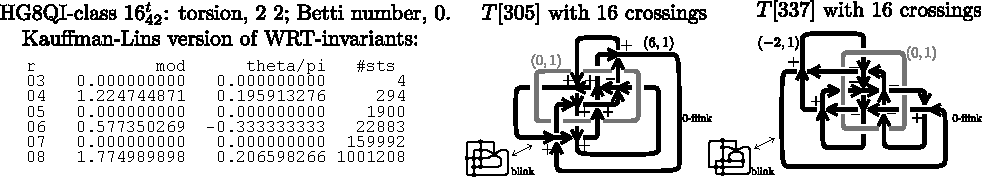
\includegraphics[width=16.0cm]{A.figs/T16_42.pdf} 
\caption{\sf Distinction on the $HG8QI$-class $16^t_{42}$:
% {\color{red} 
Homology of the six 4-covers of $T[305]$: $
[Z/2 + Z/2 + Z/2 + Z/2 + Z/114,
 Z/2 + Z/29146,
 Z/2 + Z/2 + Z/2 + Z/2 + Z/6,
 Z/2 + Z/2 + Z/2 + Z/2 + Z/6,
 Z/2 + Z/1305434,
 Z/16169 + Z]
  $.
Homology of the six 4-covers of $T[337]$: 
$
 [Z/2 + Z/2 + Z/2 + Z/6 + Z/6,
 Z/2 + Z/2 + Z/2 + Z/2 + Z/150,
 Z/2 + Z/2 + Z/2 + Z/2 + Z/150,
 Z/2 + Z/29146,
 Z/2 + Z/1305434,
 Z/16169 + Z]
$.
Therefore $T[305]$ and $T[337]$ induce non-homeomorphic 3-manifolds. 
Note that the volumes (as the Kauffman-Lins version of the WRT-invariants) do not distinguish:
volume of $T[305]$ ---32.9085657755, volume of $T[337]$ --- 32.908565776. 
Sage Execution Time (CPU time 0m1.89s, Wall time 0m4.98s).
}
% }
% Homology of the twenty three 5-covers of $T[305]$: $
% [Z/2 + Z/2 + Z/2 + Z/2 + Z/2 + Z/4 + Z/8,
%  Z/2 + Z/2 + Z/2 + Z/2 + Z/2 + Z/16 + Z,
%  Z/2 + Z/2 + Z/2 + Z/2 + Z/2 + Z/16 + Z,
%  Z/2 + Z/2 + Z/2 + Z/2 + Z/4 + Z/264,
%  Z/2 + Z/2 + Z/2 + Z/2 + Z/10,
%  Z/2 + Z/2 + Z/2 + Z/2 + Z/9576,
%  Z/2 + Z/2 + Z/2 + Z/498,
%  Z/2 + Z/2 + Z/2 + Z/1746,
%  Z/2 + Z/2 + Z/2 + Z/1746,
%  Z/2 + Z/2 + Z/4 + Z/4 + Z/32,
%  Z/2 + Z/2 + Z/4 + Z/60 + Z,
%  Z/2 + Z/2 + Z/4 + Z/64,
%  Z/2 + Z/2 + Z/4 + Z/64,
%  Z/2 + Z/2 + Z/6 + Z/12,
%  Z/2 + Z/2 + Z/18 + Z/18,
%  Z/2 + Z/2 + Z/18 + Z/18,
%  Z/2 + Z/2 + Z/24 + Z + Z,
%  Z/2 + Z/2 + Z/48870,
%  Z/2 + Z/2 + Z/49208,
%  Z/2 + Z/2 + Z/49208,
%  Z/2 + Z/6 + Z/204,
%  Z/2 + Z/6 + Z/714,
%  Z/2 + Z/22 + Z/118360]
%  $.
% Homology of the eighteen 5-covers of $T[337]$: 
% $
% [Z/2 + Z/2 + Z/2 + Z/2 + Z/2 + Z/8 + Z/56,
%  Z/2 + Z/2 + Z/2 + Z/2 + Z/2 + Z/16 + Z,
%  Z/2 + Z/2 + Z/2 + Z/2 + Z/2 + Z/16 + Z,
%  Z/2 + Z/2 + Z/2 + Z/2 + Z/4 + Z/4664,
%  Z/2 + Z/2 + Z/2 + Z/2 + Z/286,
%  Z/2 + Z/2 + Z/2 + Z/2 + Z/702,
%  Z/2 + Z/2 + Z/2 + Z/2 + Z/702,
%  Z/2 + Z/2 + Z/2 + Z/78 + Z,
%  Z/2 + Z/2 + Z/2 + Z/1104,
%  Z/2 + Z/2 + Z/4 + Z/4 + Z,
%  Z/2 + Z/2 + Z/4 + Z/20,
%  Z/2 + Z/2 + Z/4 + Z/20,
%  Z/2 + Z/2 + Z/4 + Z/324,
%  Z/2 + Z/2 + Z/4 + Z/324,
%  Z/2 + Z/2 + Z/6 + Z/12,
%  Z/2 + Z/2 + Z/24 + Z + Z,
%  Z/2 + Z/2 + Z/1530,
%  Z/2 + Z/2 + Z/58698]
% $.
% Therefore $T[305]$ and $T[337]$ induce non-homeomorphic 3-manifolds. 
% Note that the volumes (as the Kauffman-Lins version of the WRT-invariants) do not distinguish:
% volume of $T[305]$ ---32.9085657755, volume of $T[337]$ --- 32.908565776. 
% Sage Execution Time (CPU time 0m5.49s, Wall time 3m36.56s).
% }
\label{fig:T16_42}
\end{center}
\end{figure} 

\subsection{Distinguishing the 2 members of the $HG8QI$-class  $16^t_{56}$}
\begin{figure}[H]
\begin{center}
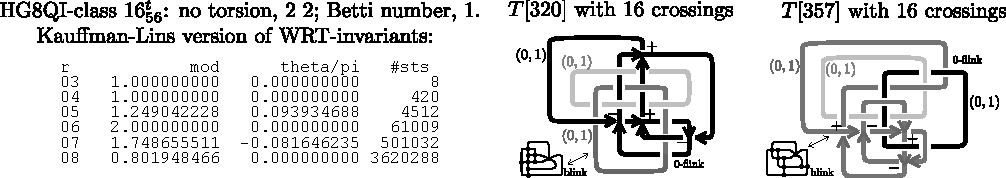
\includegraphics[width=16.0cm]{A.figs/T16_56.pdf} 
\caption{\sf Distinction on the $HG8QI$-class $16^t_{56}$:
% {\color{red}
Homology of the five 3-covers of $T[320]$: $
[Z, Z/2 + Z/34 + Z, Z/7 + Z/7 + Z, Z/37 + Z, Z/71 + Z]
$.
Homology of the five 5-covers of $T[357]$: 
$
[Z, Z/2 + Z/2 + Z/2 + Z/4 + Z, Z/2 + Z/32 + Z, Z/2 + Z/40 + Z, Z/7 + Z/7 + Z]
$.
Therefore $T[320]$ and $T[357]$ induce non-homeomorphic 3-manifolds. 
Note that the volumes also distinguish, on the contrary of the previous volumes:
volume of $T[320]$ ---29.4362635970, volume of $T[357]$ --- 29.460315997. 
Sage Execution Time (CPU time 0m1.40s, Wall time 0m2.63s).         
}
% }
% Homology of the five 5-covers of $T[320]$: $
%  [Z, Z/2 + Z/34 + Z, Z/7 + Z/7 + Z, Z/37 + Z, Z/71 + Z]
%  $.
% Homology of the five 5-covers of $T[357]$: 
% $
% [Z, Z/2 + Z/2 + Z/2 + Z/4 + Z, Z/2 + Z/32 + Z, Z/2 + Z/40 + Z, Z/7 + Z/7 + Z]
% $.
% Therefore $T[320]$ and $T[357]$ induce non-homeomorphic 3-manifolds. 
% Note that the volumes also distinguish, on the contrary of the previous volumes:
% volume of $T[320]$ ---29.4362635970, volume of $T[357]$ --- 29.460315997. 
% Sage Execution Time (CPU time 0m2.23s, Wall time 0m3.73s).
% }
\label{fig:T16_56}
\end{center}
\end{figure} 

\subsection{The 2 members of the $HG8QI$-class  $16^t_{140}$ remain a big challenge}
\begin{figure}[H]
\begin{center}
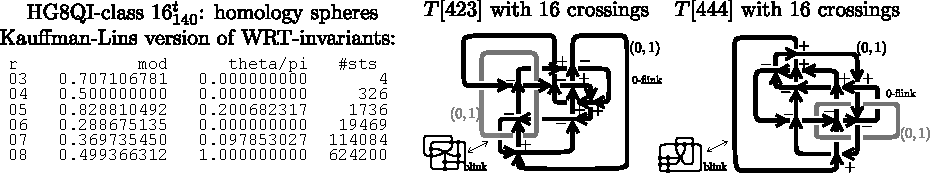
\includegraphics[width=16.0cm]{A.figs/T16_140.pdf} 
\caption{\sf Trying to distinguish the two blinks in the $HG8QI$-class $16^t_{140}$:
Inconclusive --- there are no $k$-covers for $k=2,\ldots 6$ and the search for
7-covers took more than three days without ending. We did not try $k$-covers for $k \ge 8$.
Both induced 3-manifolds have the same volume: 30.587901596. We conjecture that the
induced manifolds are non-homeomorphic.
}
\label{fig:T16_140}
\end{center}
\end{figure} 


\subsection{Distinguishing the 2 members of the $HG8QI$-class  $16^t_{141}$}
\begin{figure}[H]
\begin{center}
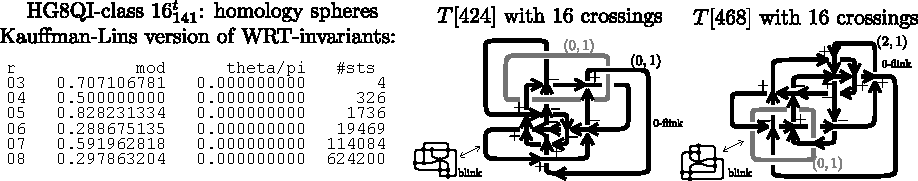
\includegraphics[width=16.0cm]{A.figs/T16_141.pdf} 
\caption{\sf Distinction on the $HG8QI$-class $16^t_{141}$:
Homology of the three 5-covers of $T[320]$: $
[Z/2 + Z/4285014, Z/2 + Z/4285014, Z/3 + Z/3 + Z/3 + Z/3]
$.
Homology of the three 5-covers of $T[357]$: 
$
[Z/2 + Z/3357564, Z/2 + Z/3357564, Z/3 + Z/3 + Z/3 + Z/3]
$.
Therefore $T[424]$ and $T[468]$ induce non-homeomorphic 3-manifolds. 
Note that the volumes (as the Kauffman-Lins version of the WRT-invariants) do not distinguish:
volume of $T[424]$ ---30.7074870213, volume of $T[468]$ --- 30.707487021. 
Sage Execution Time (CPU time 0m0.90s, Wall time 1m18.90s).
}
\label{fig:T16_141}
\end{center}
\end{figure} 


\subsection{Distinguishing the 2 members of the $HG8QI$-class  $16^t_{142}$}
\begin{figure}[H]
\begin{center}
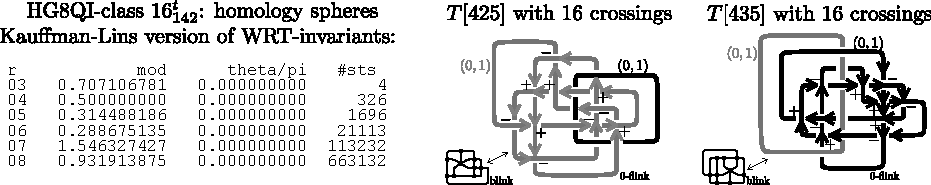
\includegraphics[width=16.0cm]{A.figs/T16_142.pdf} 
\caption{\sf Distinction on the $HG8QI$-class $16^t_{142}$:
% {\color{red}
Homology of the twenty nine 6-covers of $T[425]$:
% }
$
[Z/2 + Z/2 + Z/2 + Z/2 + Z/4,
 Z/2 + Z/2 + Z/2 + Z/2 + Z/4,
 Z/2 + Z/2 + Z/2 + Z/2 + Z/12 + Z/12 + Z,
 Z/2 + Z/2 + Z/168,
 Z/2 + Z/2 + Z/168,
 Z/2 + Z/2 + Z/12804,
 Z/2 + Z/2 + Z/12804,
 Z/2 + Z/2 + Z/42006,
 Z/2 + Z/2 + Z/42006,
 Z/3 + Z/3 + Z,
 Z/3 + Z/3 + Z,
 Z/3 + Z/3 + Z/162,
 Z/3 + Z/3 + Z/162,
 Z/3 + Z/3 + Z/1668,
 Z/3 + Z/3 + Z/1668,
 Z/3 + Z/84,
 Z/3 + Z/84,
 Z/3 + Z/990,
 Z/3 + Z/990,
 Z/3 + Z/13548,
 Z/3 + Z/13548,
 Z/3 + Z/26358,
 Z/3 + Z/26358,
 Z/4 + Z/4 + Z,
 Z/4 + Z/4 + Z,
 Z/6 + Z/6 + Z,
 Z/57 + Z/57 + Z,
 Z/7392,
 Z/7392]
$.
% {\color{red}
Homology of the twenty nine 6-covers of $T[435]$: 
% }
$
[Z/2 + Z/2 + Z/2 + Z/2 + Z/4,
 Z/2 + Z/2 + Z/2 + Z/2 + Z/4,
 Z/2 + Z/2 + Z/2 + Z/2 + Z/12 + Z/12 + Z,
 Z/3 + Z/3 + Z,
 Z/3 + Z/3 + Z,
 Z/3 + Z/468,
 Z/3 + Z/468,
 Z/3 + Z/1632,
 Z/3 + Z/1632,
 Z/3 + Z/3618,
 Z/3 + Z/3618,
 Z/3 + Z/47694,
 Z/3 + Z/47694,
 Z/4 + Z/4 + Z,
 Z/4 + Z/4 + Z,
 Z/6 + Z/6 + Z/6324,
 Z/6 + Z/6 + Z/6324,
 Z/6 + Z/6 + Z/61254,
 Z/6 + Z/6 + Z/61254,
 Z/9 + Z/9 + Z,
 Z/126 + Z/126 + Z,
 Z/4200,
 Z/4200,
 Z/10422,
 Z/10422,
 Z/13344,
 Z/13344,
 Z/14454,
 Z/14454]
$.
Therefore $T[425]$ and $T[435]$ induce non-homeomorphic 3-manifolds. 
Note that the volumes (as the Kauffman-Lins version of the WRT-invariants) do not distinguish:
volume of $T[425]$ --- 30.729338019, volume of $T[435]$ --- 30.7293380190. 
Sage Execution Time (CPU time 0m47.88s, Wall time 233m45.92s).
}
\label{fig:T16_142}
\end{center}
\end{figure} 

\subsection{Distinguishing the 2 members of the $HG8QI$-class  $16^t_{149}$}
\begin{figure}[H]
\begin{center}
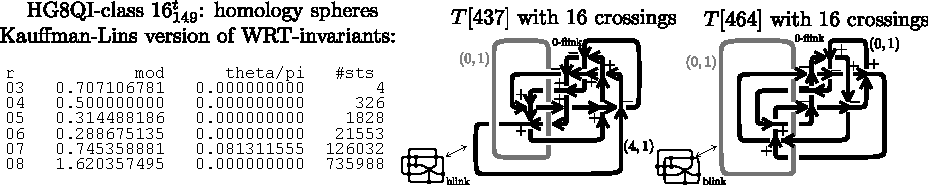
\includegraphics[width=16.0cm]{A.figs/T16_149.pdf} 
\caption{\sf Distinction on the $HG8QI$-class $16^t_{149}$:
% {\color{red}
Homology of the zero 5-covers of $T[437]$: $
[]
$.
% sage: []\\
Homology of the two 5-covers of $T[464]$: $
[Z/3 + Z/12 + Z, Z/3 + Z/12 + Z]
$.
% sage: [Z/3 + Z/12 + Z, Z/3 + Z/12 + Z]\\
Note that the volumes are distinctly different,
33.464380115 for $T[437]$ and 30.8673418910 for $T[464]$.
Therefore $T[437]$ and $T[464]$ induce non-homeomorphic 3-manifolds. 
Sage Execution Time (CPU time 0m9.18s, Wall time 34m7.37s).
}
% }
% on the contrary of the others pairs,
% we were not able to find covers after waiting various days. However,
% the volumes are distinctly different,
% 33.464380115 for $T[437]$ and 30.8673418910 for $T[464]$.
% Therefore $T[437]$ and $T[464]$ induce non-homeomorphic 3-manifolds. 
% Sage Execution Time (CPU time inconclusive, Wall time inconclusive).
% }
\label{fig:T16_149}
\end{center}
\end{figure} 


\subsection{Distinguishing the 2 members of the $HG8QI$-class  $16^t_{233}$}
\begin{figure}[H]
\begin{center}
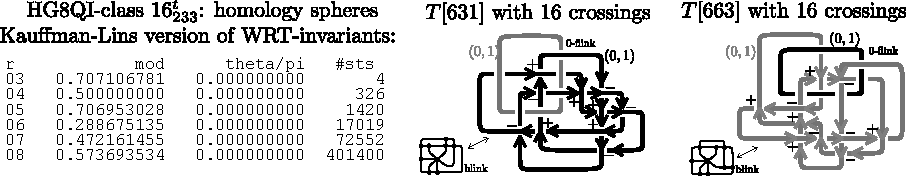
\includegraphics[width=16.0cm]{A.figs/T16_233.pdf} 
\caption{\sf Distinction on the $HG8QI$-class $16^t_{233}$:
Homology of the two 5-covers of $T[631]$: $
[Z/4 + Z/4 + Z/36 + Z/36, Z/21 + Z/21]
$.
Homology of the two 5-covers of $T[663]$: 
$
[Z/2 + Z/2 + Z/258 + Z/258, Z/171 + Z/171]
$.
Therefore $T[631]$ and $T[663]$ induce non-homeomorphic 3-manifolds. 
Note that the volumes (as the Kauffman-Lins version of the WRT-invariants) do not distinguish:
volume of $T[631]$ ---29.624669407, volume of $T[663]$ --- 29.6246694067. 
Sage Execution Time (CPU time 0m1.68s, Wall time 1m5.63s).
}
\label{fig:T16_233}
\end{center}
\end{figure} 

% \section{Appendix: SnapPy/GAP/Sage summarized sections}

\section{Conclusion}
With the exception of $16_{140}^t$, we have noticed that if blink $B'\notin \{B,-B^\star\}$,
then $B$ and $B'$ induce non-homeomorphic 3-manifolds. We do not know wheter $T[423]$ and $T[444]$
induce homeomorphic 3-manifolds or not. Our bet, to make 3-connected monochromatic blinks
conform to their induced 3-manifolds, is that they are non-homeomorphic. We leave this doubt as
a focused remaining challenge to the 3-manifold community. In the realm of the 381 members of
$T_{16}$, this is the only pair 
that is unresolved from the 11 challenging $HG8QI$-classes 
presented in \url{http://arxiv.org/abs/1305.2617}, \cite{lins2013}. Maybe we have reach the current
technological limit with this example. 
This strongly points to the research goal of finding 
still better invariants of 3-manifolds. We hope that \url{http://arxiv.org/abs/1305.4540}, \cite{lins2013B}
has something to say in this direction.

\bibliographystyle{plain}
%\bibliographystyle{is-alpha}
%\addcontentsline{toc}{bibliografia}{\MakeTextUppercase{Refer�ncias Bibliogr�ficas}}
%\bibliography{d:/slsl\3.DadosSostenes.35.ArtigosLivros.bibtexGoogleScholar/bibtexIndex.bib} % bib file is slsl.bib
%\bibliography{~/home/ricardo/Dropbox/35.ArtigosLivros.bibtexGoogleScholar/bibtexIndex.bib}
\bibliography{bibtexIndex.bib}
%\bibliography{slsl}

\begin{small}
\begin{center}
\begin{tabular}{l}
S\'ostenes L. Lins\\
Centro de Inform\'atica, UFPE \\
Av. Jorn.  Anibal Fernandes s/n\\
Recife, PE 50740-560 \\
Brazil\\
sostenes@cin.ufpe.br
\end{tabular}
\begin{tabular}{l}
Cristiana G. Huiban\\
Centro de Inform\'atica, UFPE \\
Av. Jorn.  Anibal Fernandes s/n\\
Recife, PE 50740-560 \\
Brazil\\
cmngh@cin.ufpe.br
\end{tabular}
\hspace{0mm}
\begin{tabular}{l}
Lauro D. Lins\\
AT\&T Labs Research \\
180 Park Avenue \\
Florham Park, NJ 07932 \\
USA\\
llins@research.att.com
\end{tabular}
\hspace{20mm}
\end{center}
\end{small}

\end{document}

% \printindex